% Options for packages loaded elsewhere
\PassOptionsToPackage{unicode}{hyperref}
\PassOptionsToPackage{hyphens}{url}
\PassOptionsToPackage{dvipsnames,svgnames,x11names}{xcolor}
%
\documentclass[
  12pt,
  a4paper, twoside]{book}
\usepackage{amsmath,amssymb}
\usepackage{iftex}
\ifPDFTeX
  \usepackage[T1]{fontenc}
  \usepackage[utf8]{inputenc}
  \usepackage{textcomp} % provide euro and other symbols
\else % if luatex or xetex
  \usepackage{unicode-math} % this also loads fontspec
  \defaultfontfeatures{Scale=MatchLowercase}
  \defaultfontfeatures[\rmfamily]{Ligatures=TeX,Scale=1}
\fi
\usepackage{lmodern}
\ifPDFTeX\else
  % xetex/luatex font selection
\fi
% Use upquote if available, for straight quotes in verbatim environments
\IfFileExists{upquote.sty}{\usepackage{upquote}}{}
\IfFileExists{microtype.sty}{% use microtype if available
  \usepackage[]{microtype}
  \UseMicrotypeSet[protrusion]{basicmath} % disable protrusion for tt fonts
}{}
\makeatletter
\@ifundefined{KOMAClassName}{% if non-KOMA class
  \IfFileExists{parskip.sty}{%
    \usepackage{parskip}
  }{% else
    \setlength{\parindent}{0pt}
    \setlength{\parskip}{6pt plus 2pt minus 1pt}}
}{% if KOMA class
  \KOMAoptions{parskip=half}}
\makeatother
\usepackage{xcolor}
\usepackage{longtable,booktabs,array}
\usepackage{calc} % for calculating minipage widths
% Correct order of tables after \paragraph or \subparagraph
\usepackage{etoolbox}
\makeatletter
\patchcmd\longtable{\par}{\if@noskipsec\mbox{}\fi\par}{}{}
\makeatother
% Allow footnotes in longtable head/foot
\IfFileExists{footnotehyper.sty}{\usepackage{footnotehyper}}{\usepackage{footnote}}
\makesavenoteenv{longtable}
\usepackage{graphicx}
\makeatletter
\def\maxwidth{\ifdim\Gin@nat@width>\linewidth\linewidth\else\Gin@nat@width\fi}
\def\maxheight{\ifdim\Gin@nat@height>\textheight\textheight\else\Gin@nat@height\fi}
\makeatother
% Scale images if necessary, so that they will not overflow the page
% margins by default, and it is still possible to overwrite the defaults
% using explicit options in \includegraphics[width, height, ...]{}
\setkeys{Gin}{width=\maxwidth,height=\maxheight,keepaspectratio}
% Set default figure placement to htbp
\makeatletter
\def\fps@figure{htbp}
\makeatother
\setlength{\emergencystretch}{3em} % prevent overfull lines
\providecommand{\tightlist}{%
  \setlength{\itemsep}{0pt}\setlength{\parskip}{0pt}}
\setcounter{secnumdepth}{5}
\ifLuaTeX
\usepackage[bidi=basic]{babel}
\else
\usepackage[bidi=default]{babel}
\fi
\babelprovide[main,import]{finnish}
% get rid of language-specific shorthands (see #6817):
\let\LanguageShortHands\languageshorthands
\def\languageshorthands#1{}
\usepackage{booktabs}
\usepackage[T1]{fontenc}
\usepackage[utf8]{inputenc}
\usepackage{color}
\usepackage{xspace}
\usepackage{tikz-cd}
\usepackage{mathtools}
\usepackage{mathrsfs}
\usepackage{comment}
\usepackage{commath}
\usepackage{pict2e}
\usepackage{float}
\usepackage{array, makecell}
\usepackage{amsthm}														% 
\usepackage{amsmath}
%\usepackage[tagpdf]{axessibility} 
\usepackage[ruled,vlined,shortend]{algorithm2e} 
\usepackage{graphicx}
\usepackage{multicol}
\usepackage{gensymb}
%\usepackage[a-3b]{pdfx}
\graphicspath{ {./images/} }
\usetikzlibrary{shapes.geometric,arrows}
\def\TikZ{Ti\emph{k}Z\ }
\renewcommand{\algorithmcfname}{Algoritmi}
\usepackage{geometry}
\geometry{
    a4paper,
    total={150mm,237mm},
    left=30mm,
    top=30mm,
    }
\newcommand{\tekija}{{Lasse Rintakumpu}}
\newcommand{\titteli}{{}} 
\newcommand{\otsikko}{{Hiukassuodin- ja hiukassiloitinalgoritmit sekä niiden soveltaminen AoA-menetelmään perustuvassa Bluetooth-sisätilapaikannuksessa}} 
\newcommand{\tutkielma}{{Pro gradu }}
\newcommand{\aika}{{Maaliskuu 2024}} 
\newcommand{\paaaine}{{Tilastotiede}} 
\newcommand{\ohjaaja}{{Ohjaajan titteli (Prof./Dos./FT) ja nimi }} %
\newcommand{\tarkastaja}{{Toisen tarkastajan titteli (Prof./Dos./FT) ja nimi}} 
\ifLuaTeX
  \usepackage{selnolig}  % disable illegal ligatures
\fi
\usepackage[]{natbib}
\bibliographystyle{plainnat}
\IfFileExists{bookmark.sty}{\usepackage{bookmark}}{\usepackage{hyperref}}
\IfFileExists{xurl.sty}{\usepackage{xurl}}{} % add URL line breaks if available
\urlstyle{same}
\hypersetup{
  pdflang={fi},
  colorlinks=true,
  linkcolor={blue},
  filecolor={Maroon},
  citecolor={blue},
  urlcolor={blue},
  pdfcreator={LaTeX via pandoc}}

\author{}
\date{\vspace{-2.5em}}

\begin{document}

\pagenumbering{roman}
\pagestyle{empty}

\begin{center}

\includegraphics[width=10cm]{UTU_logo_FI}
\end{center}

\vspace{3.0cm}
\begin{center}\large
{\sc \otsikko} 
\end{center}

\vspace{0.5cm}
\begin{center}
\titteli \tekija
\end{center}

\vspace{0.5cm}
\begin{center}
\tutkielma -tutkielma\\
\aika
\end{center}

\vspace{2.5cm}
\begin{center}
\begin{tabular}{l}
Tarkastajat:\\
\ohjaaja \\
\tarkastaja
\end{tabular}
\end{center}

\vspace{2.5cm}
\begin{center}
MATEMATIIKAN JA TILASTOTIETEEN LAITOS
\end{center}

\newpage\null

\vspace{22cm}

\noindent Turun yliopiston laatujärjestelmän mukaisesti tämän julkaisun alkuperäisyys on tarkastettu Turnitin OriginalityCheck-järjestelmällä

\cleardoublepage

\noindent
TURUN YLIOPISTO \newline
Matematiikan ja tilastotieteen laitos\newline

\noindent \textsc{\tekija}: \otsikko \newline
\tutkielma-tutkielma, X s. \newline
\paaaine \newline
\aika
\par\noindent{\rule{\textwidth}{.2mm}} \newline


\vspace{4mm}\noindent Tutkielmassa esitetään hiukassuodin- ja hiukassiloitinalgoritmien teoria Bayesilaisessa tilastotieteellisessä viitekehyksessä. Lisäksi tutkielmassa käsitellään hiukassuotimien varianssin estimointia.

\vspace{4mm}\noindent Empiirisenä esimerkkinä tutkielmassa tarkastellaan hiukassuodin- ja hiukassiloitinalgoritmien käyttöä AoA-teknologiaan perustuvassa Bluetooth-sisätilapaikannusratkaisussa.

\vspace{4mm}\noindent Asiasanat: SMC-menetelmät, Monte Carlo -menetelmät, sekventiaalinen Monte Carlo, suodinongelma, hiukassuodin, hiukassiloitin, SIR-algoritmi, sisätilapaikannus, BLE, AoA, triangulaatio, Bayesilainen päättely

\cleardoublepage

\cleardoublepage

\pagestyle{plain} 
\pagenumbering{arabic} 

{
\hypersetup{linkcolor=blue}
\setcounter{tocdepth}{2}
\tableofcontents
}
\setlength\parindent{24pt}
\setlength\parskip{3pt}

\chapter{Johdanto}

SMC-menetelmät (sequential Monte Carlo -mentelmät) ovat joukko Monte Carlo -algoritmeja, joiden avulla voidaan ratkaista ns. suodinongelma, kun ongelma on epälineaarinen ja/tai ongelmaan liittyvä kohina ei noudata normaalijakaumaa. SMC-menetelmille on lukuisia sovellutuksia esimerkiksi Bayesilaisessa tilastotieteessä, fysiikassa ja robotiikassa.

Tämän tutkielman tavoitteena on esittää pääpiirteittäin SMC-menetelmien teoria sekä joitakin menetelmäperheeseen kuuluvia algoritmeja. Tutkielman ensimmäisessä alaluvussa kuvataan yleisellä tasolla sekä suodinongelma että sen ratkaisujen historiaa. Toisessa alaluvussa käsitellään joitakin Monte Carlo -menetelmiin liittyviä yleisiä tuloksia. Kolmannessa alaluvussa esitellään Bayesilainen viitekehys suodinongelmalle, jonka pohjalta neljännessä alaluvussa kuvataan SIR-algoritmina tunnettu SMC-menetelmä. Tutkielman lopussa tarkastellaan menetelmien käyttöä sisätilapaikannussovelluksessa.

Hiukassuodin- sekä hiukassiloitinalgoritmien osalta tutkielman esitykset seuraavat erityisesti Simo Särkän kirjaa \textit{Bayesian Filtering and Smoothing} (2013), Fredrik Gustafssonin artikkelia ``Particle Filter Theory and Practice with Positioning Applications'' (2010) sekä Olivier Cappén, Simon J. Godsillin ja Eric Moulines'n artikkelia ``An overview of existing methods and recent advances in sequential Monte Carlo'' (2007). Hiukassuotimien varianssin estimointi seuraa artikkeleita TODO.

\section{Suodinongelma}

Stokastisten prosessien teoriassa suodinongelmaksi kutsutaan tilannetta, jossa halutaan muodostaa keskineliövirheen mielessä paras mahdollinen estimaatti jonkin järjestelmän tilan arvoille, kun ainoastaan osa tiloista voidaan havaita ja/tai havaintoihin liittyy kohinaa. Tavoitteena on toisin sanoen laskea jonkin prosessin posteriorijakauma kyseisten havaintojen perusteella. Ongelmaa havainnollistaa kaavio (\ref{mallikaavio}).

\begin{equation}\label{mallikaavio}
\begin{tikzcd}
x_1 \arrow[d] \arrow[r] & x_2 \arrow[d] \arrow[r] & x_3 \arrow[d] \arrow[r] & \ldots & \makebox[\widthof{$ \text{havainnot}$}]{$\text{piilossa olevat tilat}$} \\
y_1  & y_2  & y_3  & \ldots & \makebox[\widthof{$ \text{havainnot}$}]{$\text{havainnot}$}
\end{tikzcd}
\end{equation}

Tässä tutkielmassa keskitytään erityisesti epälineaarisen ns. Markovin piilomallin posteriorijakauman Bayesilaiseen ratkaisuun. Ongelmassa tiedetään, miten havaitut muuttujat \(y_k\) kytkeytyvät ``piilossa oleviin'' tilamuuttujiin \(x_k\) sekä osataan sanoa jotain tilamuuttujien todennäköisyyksistä. Oletetaan myös, että piilossa oleville tiloille \(X_k\) pätee Markov-ominaisuus, jolloin kutakin hetkeä seuraava tila \(x_{k+1}\) riippuu menneistä tiloista \(x_{1:k}\) ainoastaan tilan \(x_k\) välityksellä. Lisäksi havaittu tila \(y_k\) riippuu tiloista \(x_{k}\) ainoastaan jonkin \(x_k\):n funktion kautta. Kun aika-avaruus on diskreetti ja ajanhetkellä \(k=\{1,\ldots,t\}\) piilossa olevan prosessin tilaa merkitään \(x_k\) ja havaittua prosessia \(y_k\), saadaan mallit

\begin{align}
&\label{malli-1} x_{k+1} = f(x_k, \nu_k),\\
&\label{malli-2} y_{k} = h(x_k)+e_k.
\end{align}

Lisäksi tiedetään prosessin alkuhetken jakauma \(x_0 \sim p_{x_{0}}\), tähän liittyvän kohinaprosessin jakauma \(\nu_k \sim p_{\nu_{k}}\) sekä malliin \(y_k\) liittyvä kohina \(e_k \sim p_{e_k}\). Koska SMC-algoritmit pyrkivät ratkaisemaan juurikin epälineaarisen, ei-Gaussisen suodinongelman, voivat funktiot \(f(\cdot)\) ja \(h(\cdot)\) olla epälineaarisia eikä kohinan tarvitse olla normaalijakautunutta.

Mallit voidaan esittää myös yleisemmässä jakaumamuodossa

\begin{align}
&\label{malli-3} x_{k+1} \sim p(x_{k+1}|x_k),\\
&\label{malli-4} y_{k} \sim p(y_k|x_k).
\end{align}

Tutkielman teoriaosassa käytetään ensisijaisesti yhtälöiden (\ref{malli-3}) ja (\ref{malli-4}) muotoilua. Empiirisessä osassa palataan yhtälöiden (\ref{malli-1}) ja (\ref{malli-2}) muotoiluun.

Suodinongelmaa lähellä on myös ns. tasoitusongelma (smoothing problem), jossa ollaan kiinnostuneita prosessin \(x_k\) posteriorijakaumasta \(p(x_k|y_k)\) jokaisena ajanhetkenä \(\{1,\ldots,k\}\) ei ainoastaan haluttuna ajanhetkenä \(k\). Tämä tutkielma keskittyy yksin suodinongelman ratkaisemiseen, mutta huomioitavaa on, että SMC-algoritmit näyttävät ratkaisevan tasoitusongelman ilmaiseksi. Tähän liittyy kuitenkin joidenkin mallien kohdalla mahdollista epätarkkuutta, joten tarvittaessa tasoitusongelma pitää ratkaista erikseen.

\section{Notaatioista}

Tässä tutkielmassa käytetään seuraavia notaatioita. TODO.

\section{Suodin- ja siloitteluongelmien historiaa}

Tämä alaluku esittää pääpiirteittään suodinongelmalle esitettyjen ratkaisujen historian. Lineaarisen suodinongelman osalta alaluku noudattaa Dan Crisanin artikkelia ``The stochastic filtering problem: a brief historical account'' (2014) sekä Mohinder S. Grewalin ja Angus P. Andrewsin artikkelia ``Applications of Kalman Filtering in Aerospace 1960 to the Present'' (2010). SMC-menetelmien osalta lähteenä toimii Cappé \&al (2007).

Suodinongelma nousi esille insinööritieteiden sekä sotateollisuuden käytännön ongelmista 2. maailmansodan aikana, vaikkakin suodinongelman diskreetin ajan ratkaisut juontavat jo Andrei N. Kolmogorovin 30-luvun artikkeleihin. Jatkuvan ajan tilanteessa ensimmäisen optimaalisen, kohinan sallivan suotimen esitti matemaatikko, kybernetiikan kehittäjä Norbert Wiener. Wiener-suotimena tunnettua ratkaisuaan varten Wiener muotoili seuraavat kolme ominaisuutta, jotka prosessin \(X\) estimaatin \(\hat{X}_t\) pitää toteuttaa.

\begin{enumerate}
\vspace{\baselineskip}
\item \textit{Kausaliteetti}: $X_t$ tulee estimoida käyttäen arvoja $Y_s$, missä $s \leq t$.
\item \textit{Optimaalisuus}: $X_t$:n estimaatin $\hat{X}_t$ tulee minimoida keskineliövirhe $\mathbb{E}[(X-\hat{X}_t)^2]$.
\item \textit{On-line -estimointi}: Estimaatin $\hat{X}_t$ tulee olla saatavissa minä hyvänsä ajanhetkenä $t$. 
\vspace{\baselineskip}
\end{enumerate}

Wiener sovelsi ratkaisussaan stationaaristen prosessien spektriteoriaa. Tulokset julkaistiin salaisina Yhdysvaltojen asevoimien tutkimuksesta vastanneen National Defense Research Committeen (NDRC) raportissa vuonna 1942. Tutkimus tunnettiin sodan aikana lempinimellä ``Keltainen vaara'' sekä painopaperinsa värin että vaikeaselkoisuutensa vuoksi. Myöhemmin Wiener esitti tuloksensa julkisesti kirjassaan \textit{Extrapolation, Interpolation and Smoothing of Stationary Time Series} (1949). Wienerin alkuperäiset kolme perusperiaatetta päteveät edelleen kaikille suodinongelman ratkaisuille, myös SMC-menetelmille.

Kenties tärkein ja varmasti tunnetuin lineaariseen suodinongelman ratkaisu on Kalman-suodin. Suotimen kehittivät R.E. Kalman ja R.S. Bucy 1950- ja 60-lukujen taitteessa Yhdysvaltain kylmän sodan kilpavarustelutarpeisiin perustetussa Research Institute for Advanced Studies -tutkimuslaitoksessa (RIAS). Kalman-suodin on suodinongelman diskreetin ajan ratkaisu, kun taas Kalman-Bucy-suodin on jatkuvan ajan ratkaisu. Kohinan ollessa normaalijakautunutta on Kalman-suodin Wiener-suotimen tavoin lineaarisen suodinongelman optimaalinen ratkaisu. Wiener-suotimella ja Kalman-suotimella on kuitenkin erilaiset oletukset, minkä vuoksi erityisesti säätö- ja paikannussovelluksissa Kalman-suotimen käyttö on luontevampaa. Suotimien oletuksia ja oletusten välisiä eroja ei käsitellä tässä tutkielmassa, kuten ei käsitellä myöskään Kalman-suotimen formaalia yhteyttä SMC-menetelmiin.

Kalman-suodinta voidaan soveltaa myös epälineaarisessa tapauksessa, kunhan suodinongelman funktiot \(f(\cdot)\) ja \(h(\cdot)\) ovat derivoituvia ja niihin liittyvä kohina oletetaan normaalijakautuneeksi. Tätä ratkaisua kutsutaan laajennetuksi Kalman-suotimeksi (extended Kalman filter, EKF). Suodin kehitettiin 60-luvulla NASA:n Apollo-ohjelman tarpeisiin, vaikkakin itse avaruusalusten laitteistot hyödynsivät lentoratojen laskennassa Kalman-suotimen perusversiota. Laajennetun Kalman-suotimen toimintaperiaate perustuu epälineaaristen funktioiden linearisointiin Taylorin kehitelmän avulla kulloisenkin estimaatin ympärillä. Laajennettu Kalman-suodin on erityisesti paikannussovellusten \textit{de facto} -suodinstandardi, mutta suodin ei kuitenkaan ole epälineaarisen ongelman optimaalinen estimaattori.

Kalman-suotimesta on lisäksi olemassa lukuisia muita epälineaarisiin ongelmiin soveltuvia laajennuksia, muun muassa paikkaratkaisun Kalman-suodin (position Kalman filter, PKF), hajustamaton Kalman-suodin (unscented Kalman filter, UKF) ja tilastollisesti linearisoitu Kalman-suodin (statistically linearized Kalman filter, SLF). Kuitenkin jos prosessin \(X\) mallia ei tunneta tarkasti tai kohinaa ei voida olettaa normaalijakautuneeksi, ovat sekventiaaliset Monte Carlo -menetelmät Kalman-suotimen johdannaisia parempia ratkaisuja. Vaikka tila-avaruuden dimensioiden kasvaessa kasvaa myös SMC-menetelmien vaatima laskentateho, ovat SMC-menetelmät aina sitä parempia mitä epälineaarisempia mallit ovat ja mitä kauempana normaalijakaumasta kohina on. Viimeisten vuosikymmenten aikana myös laskennan teho on kasvanut merkittävästi samalla kun laskennan hinta on vastaavasti romahtanut, mikä puoltaa Monte Carlo -menetelmien käyttöä entistä useammissa ongelmissa.

Joitakin suodinongelman rekursiivisia Monte Carlo -ratkaisuja löytyy jo 1950\textendash 70-luvuilta, erityisesti säätöteoriaan piiristä. Olennainen nykyalgoritmeihin periytynyt oivallus varhaisissa suodinalgoritmeissa oli tärkeytysotannan käyttö halutun jakaumaestimaatin laskennassa. Tärkeytysotanta-algoritmiin voidaan turvautua, kun emme pysty suoraan tekemään havaintoja jostakin jakaumasta \(p\) ja teemme sen sijaan havaintoja jakaumasta \(q\), joita painotamme niin, että tuloksena saadaan jakauman \(p\) harhaton estimaatti. Algoritmi on kuvattu tarkemmin tutkielman alaluvussa 2.

Tärkeysotantaa käyttävä suodinongelman ratkaiseva SIS-algoritmi (sequential importance sampling) ei kuitenkaan vielä 70-luvulla löytänyt suurta käytännön suosiota. Osin tämä johtui puutteellisesta laskentatehosta, mutta algoritmi kärsi myös otosten ehtymisenä (sample impoverishment) tunnetusta ongelmasta. Monissa ongelmissa SIS-algoritmia käytettäessä suuri osa painoista päätyy vain tietyille partikkeleille, jolloin vastaavasti suuri osa partikkeleista ei enää estimoi haluttua jakaumaa. Tähän ongelmaan palataan myöhemmin.

Merkittävän ratkaisun ehtymisongelmaan esittivät Gordon, Salmond ja Smith artikkelissaan ``Novel approach to nonlinear/non-Gaussian Bayesian state estimation'' (1993). Artikkelin ratkaisu kulki nimellä ``bootstrap filter'', saapasremmisuodin. Saapasremmisuodin vältti ehtymisen uudellenotannalla, jossa matalapainoiset partikkelit korvattiin otoksilla korkeapainoisemmista partikkeleista. Ratkaisussa painot eivät myöskään riipu partikkelien aiemmista poluista vaan ainoastaan havaintojen uskottavuusfunktiosta. Vastaavaa ratkaisua käytetään tämän tutkielman uudemmassa SIR-algoritmissa (sampling importance resampling), jossa myös uudelleenotantaan sovelletaan tärkeytysotantaa.

SMC-menetelmissä stokastisen prosessin posteriorijakauman esittämiseen käytettyjä otoksia kutsutaan myös partikkeleiksi ja menetelmiä hiukassuotimiksi. Erityisesti myöhemmin esitettävää SIR-algoritmia kutsutaan usein hiukkassuotimeksi. Tässä tutkielmassa pyritään korostamaan suotimien yhteyttä Monte Carlo -algoritmeihin ja käytetään siksi yleisempää termiä SMC-menetelmät. Termiä hiukkassuodin käytti ensimmäisen kerran Del Moral artikkelissa ``Nonlinear Filtering: Interacting Particle Resolution'' (1996), SMC-menetelmät termiä Liu ja Chen artikkelissa ``Sequential Monte Carlo Methods for Dynamic Systems'' (1998).

\section{Monte Carlo -menetelmistä}

Tässä alaluvussa kuvataan lyhyesti SMC-menetelmissä käytettävien Monte Carlo -menetelmien perusperiaate todennäköisyysjakauman estimoinnissa. Lisäksi esitetään tärkeytysotanta-algoritmi (importance sampling), jonka tarkoituksena on estimoida harhattomasti jakaumaa \(p(x|y_{1:k})\), josta emme voi suoraan tehdä otoksia, mutta jota voimme approksimoida toisella jakaumalla \(q\). Esitykset noudattavat Särkkää (2013).

\subsection{Monte Carlo -approksimaatio}

Bayesilaisessa päättelyssä ollaan yleisesti kiinnostuttu laskemaan johonkin posteriorijakaumaan \(p\) liittyvää odotusarvoa

\begin{align}
\mathbb{E}[g(x)|y_{1:k}]=\int g(x)p(x|y_{1:k})dx,
\end{align}

\noindent missä g on tila-avaruuden mielivaltainen funktio ja \(p(x|y_{1:t})\) on havaintoihin \(\{y_1,\ldots,y_k\}\) liittyvä \(x\):n posterioritiheysjakauma. Odotusarvo on laskettavissa suljetussa muodossa vain harvoissa tapauksissa, suodinongelman kohdalla silloin, kun kyseessä on lineaarinen ja Gaussinen malli. Odotusarvoa voidaan kuitenkin approksimoida niin sanoituilla Monte Carlo -menetelmillä. Menetelmien perusperiaate on tehdä riippumattomia otoksia estimoitavasta jakaumasta ja laskea haluttu odotusarvo otosten avulla. Jos tehdään \(N\) otosta jakaumasta \(x^i\sim p(x|y_{1:t})\), missä \(i=\{1,\ldots,N\}\) saadaan näiden otosten avulla laskettua odotusarvon estimaatti

\begin{align}
\mathbb{E}[g(x)|y_{1:k}]\simeq\frac{1}{N}\sum_{i=1}^N g(x^i).
\end{align}

Monte Carlo -estimaatti konvergoi keskeisen raja-arvolauseen nojalla ja sen estimointivirheen voidaan osoittaa olevan luokkaa \(O(\frac{1}{\sqrt{N}})\) riippumatta tilamuuttujan \(x\) dimensiosta. SMC-menetelmät hyödyntävät Monte Carlo -estimointia sekventiaalisesti, jolloin estimaatti lasketaan rekursiivisesti kullekin ajanhetkelle \(k=\{1,\ldots, t\}\). Tähän palataan alaluvuissa 3 ja 4.

\subsection{Tärkeytysotanta}

Tilanteessa, jossa Monte Carlo -otoksia ei voida tehdä suoraan jakaumasta \(p\), voidaan hyödyntää jakaumaa \(p\) approksimoivaa tärkeytys- tai ehdotusjakaumaa \(q(x|y_{1:k})\) sekä ns. tärkeytysotantaa. Oletetaan, että tunnetaan priorijakauma \(p(x)\) ja on olemassa havaintomalli \(p(y_{1:k}|x)\) sekä valittu ehdotusjakauma \(q(x|y_{1:k})\), josta voidaan tehdä otoksia. Ehdotusjakaumalta edellytetään lisäksi, että sen kantaja on suurempi tai yhtä suuri kuin jakauman \(p(x|y_{1:k})\) ja että se saa nollasta poikkeavia arvoja kaikkialla missä \(p(x|y_{1:k})\) saa nollasta poikkeavia arvoja. Kirjoitetaan halutun posteriorijakauman odotusarvo integraalina

\begin{align}
\int g(x)p(x|y_{1:k})dx=\int g(x)\frac{p(x|y_{1:k})}{q(x|y_{1:k})}q(x|y_{1:k})dx,
\end{align}

\noindent jolle voidaan muodostaa Monte Carlo -approksimaatio tekemällä \(N\) otosta jakaumasta \(x^i \sim q(x|y_{1:k})\).

Muodostetaan näin odotusarvo

\begin{align}
\mathbb{E}[g(x)|y_{1:k}]\simeq\frac{1}{N}\sum_{i=1}^N\frac{p(x^i|y_{1:k})}{q(x^i|y_{1:k})}g(x^i)=\sum_{i=1}^Nw^ig(x^i),
\end{align}

\noindent missä \(g(x)\) on jokin estimoinnissa hyödyllinen, mielivaltainen funktio. Tutkielmassa käytetty notaatio \(x_k^i\) viittaa ajanhetken \(k\) partikkeliin \(i\), missä \(i=\{1,\ldots,N\}\). Tärkeytysotantaa kuvaa nyt algoritmi (\ref{tarkeytysotanta-algo}). Kun posteriorijakauman estimaatti muodostetaan kyseisellä algoritmilla voidaan tulos kirjoittaa

\begin{align}
\hat{p}(x|y_{1:k})=\sum_{i=1}^{N}w^i \delta(x-x^i),
\end{align}

\noindent missä \(\delta(x)\) on Diracin deltafunktio.

\begin{algorithm}[H]
\label{tarkeytysotanta-algo}
\DontPrintSemicolon
\Begin{
  \For{$i=1,2,\ldots,N$}{
    \Begin{Otetaan $N$ otosta ehdotusjakaumasta $x^i \sim q(x|y_{1:k}).$}
    \Begin{Lasketaan normalisoimattomat painot $w_*^i= p(y_{1:k}|x^i)p(x^i)/q(x^i|y_{1:k}).$ \newline ja normalisoidut painot $w^i=w_*^i/\sum_{j=1}^Nw_*^j$.}
    \Begin{Estimoidaan $p$ laskemalla tiheydelle approksimaatio $\mathbb{E}[g(x)|y_{1:k}]\simeq\sum_{i=1}^Nw^ig(x^i)$.}
    } 
  }  
\caption{Tärkeytysotanta}
\end{algorithm}

\subsection{Sekventiaalinen Monte Carlo}

TODO/WTF?

\section{Bayesilainen suodin}

Suodinongelmassa ollaan kiinnostuttu tilavektorin posteriorijakauman \(p(x_k|y_{1:k})\) estimoinnista. Tässä alaluvussa käydään läpi yleinen rekursiivinen, Bayesilainen posteriorijakauman laskenta. Tällaista suodinongelman ratkaisua kutsutaan myös Bayesilaiseksi suotimeksi. Koska epälineaarisessa, ei-normaalijakautuneessa tilanteessa rekursiota ei voida laskea analyyttisesti, pitää estimoinnissa käyttää numeerisia menetelmiä. SMC-menetelmissä tämä tarkoittaa jakauman sekventiaalista Monte Carlo -approksimointia, jonka toteutus esitetään alaluvun 4 algoritmissa. Molemmat esitykset noudattavat Gustafssonia (2010).

Bayesilainen ratkaisu tilavektorin posteriorijakauman estimaatille \(\hat{p}(x_k|y_{1:k})\) saadaan seuraavalla rekursiolla (käydään läpi jokaiselle ajanhetkelle \(k=\{1,\ldots,t\}\)). Lasketaan ensin

\begin{align}\label{bayes-paivitys}
p(x_k|y_{1:k}) = \frac{p(y_k|x_k)p(x_k|y_{1:k-1})}{p(y_k|y_{1:k-1})},
\end{align}

\noindent joka saadaan suoraan Bayesin kaavasta \(P(A|B)=P(B|A)P(A)/P(B)\). Normalisointivakio lasketaan integraalina

\begin{align}\label{bayes-normalisointi}
p(y_k|y_{1:k-1})=\int_{\mathbb{R}^{n_x}}p(y_k|x_k)p(x_k|y_{1:k-1})\mathop{dx_k},
\end{align}

\noindent joka saadaan kokonaistodennäköisyyskaavasta \(P(A)=\mathbb{E}[P(A|X)]=\int_{-\infty}^{\infty}P(A|X=x)f_X(x)\mathop{dx}\). Merkintä \({R}^{n_x}\) vastaa tässä piilossa olevan tilavektorin dimensiota \(n\).

Lopuksi lasketaan päivitysaskel ajalle, joka saadaan edelleen kokonaistodennäköisyydellä

\begin{align}\label{bayes-aikapaivitys}
p(x_{k+1}|y_{1:k})=\int_{\mathbb{R}^{n_x}}p(x_{k+1}|x_k)p(x_k|y_{1:k})\mathop{dx_k}.
\end{align}

\noindent Rekursion avulla voimme laskea jakauman \(p(x_k|y_{1:k})\) estimaatti käymällä rekursion läpi \(k\) kertaa.

\section{Bayesilainen siloitin}

TODO

See Figure \ref{fig:nice-fig}.

\begin{figure}

{\centering 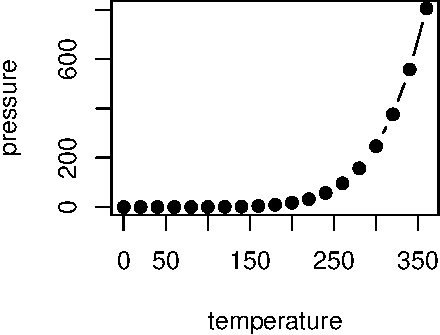
\includegraphics[width=0.8\linewidth]{output/figures/nice-fig-1} 

}

\caption{Here is a nice figure!}\label{fig:nice-fig}
\end{figure}

Don't miss Table \ref{tab:nice-tab}.

\begin{table}

\caption{\label{tab:nice-tab}Here is a nice table!}
\centering
\begin{tabular}[t]{rr}
\toprule
temperature & pressure\\
\midrule
0 & 0.0002\\
20 & 0.0012\\
40 & 0.0060\\
60 & 0.0300\\
80 & 0.0900\\
\addlinespace
100 & 0.2700\\
120 & 0.7500\\
140 & 1.8500\\
160 & 4.2000\\
180 & 8.8000\\
\bottomrule
\end{tabular}
\end{table}

\section{Kalman-suotimen ja hiukassuotimen eroista}

TODO

\chapter{Hiukassuotimet}

\section{Saapasremmisuodin}

\section{SIR-algoritmi}

Tässä alaluvussa esitetään SMC-menetelmiin kuuluva SIR-algoritmi, epälineaarisen suodinongelman ratkaisemiseksi. Algoritmi on numeerinen toteutus alaluvussa 3 kuvatusta Bayesilaisesta suotimesta. Esitetty algoritmi perustuu Gustafssoniin (2010).

Algoritmi alustetaan jakaumasta \(x_1^i\sim p_{x_0}\) generoiduilla \(N\)-kappaleella partikkeleita. Jokaiselle partikkelille annetaan alustuksessa sama paino \(w_{1|0}^i=1/N\). Algoritmi suoritetaan jokaiselle partikkelille \(i=\{1,2,\ldots,N\}\) jokaisella ajanhetkellä \(k=\{1,2,\ldots,t\}\).

Seuraava toistetaan jokaiselle ajanhetkelle \(k=\{1,2,\ldots,t\}\). Algoritmin ensimmäisessä vaiheessa päivitetään painot yhtälön (\ref{painopaivitys}) mukaan.

\begin{align}\label{painopaivitys}
w^i_{k|k}=\frac{1}{c_k}w^i_{k|k-1}p(y_k|x^i_k).
\end{align}

\noindent Tämä vastaa yllä esitetyn Bayes-suotimen päivitysvaihetta (\ref{bayes-paivitys}). Normalisointipaino \(c_k\) lasketaan puolestaan yhtälöstä (\ref{normalisointi}), mikä vastaa Bayes-suotimen normalisointivakion laskemista (\ref{bayes-normalisointi}) ja asettaa painojen summaksi \(\sum_{i=1}^Nw^i_{k|k}=1\).

\begin{align}\label{normalisointi}
c_k=\sum_{i=1}^{N}w_{k|{k-1}}^ip(y_k|x_k^i).
\end{align}

\noindent Seuraavassa vaiheessa estimoidaan \(p\) laskemalla tiheyden \(p(x_{1:k}|y_{1:k})\) Monte Carlo -estimaatti yhtälön (\ref{p-estimaatti}) perusteella

\begin{align}\label{p-estimaatti}
\hat{p}(x_{1:k}|y_{1:k})=\sum_{i=1}^{N}w_{k|k}^i \delta(x_{1:k}-x_{1:k}^i).
\end{align}

Tämän jälkeen suoritetaan valinnainen uudelleenotanta. Uudelleenotanta voidaan tehdä jokaisella askeleella tai efektiivisen otoskoon perusteella alla kuvatun kynnysarvoehdon \(\hat{N}_{eff}< N_{th}\) täyttessä, jolloin uudelleenotantaa kutsutaan adaptiiviseksi uudelleenotannaksi. Tällaista uudelleenotantaa hyödynnetään esitetyssä algoritmissa (\ref{sir}) . Uudelleenotantaa tarkastellaan lähemmin alaluvussa 4.1.2.
Lopuksi päivitetään aika (jos \(k < t\)), luodaan uudet ennusteet partikkeleille ehdotusjakaumasta (\ref{ehdotusjakauma})

\begin{align}\label{ehdotusjakauma}
x_{k+1}^i\sim q(x_{k+1}|x_k^i,y_{k+1})
\end{align}

\noindent ja päivitetään partikkelien painot tärkeytysotannalla (\ref{tarkeytys}), sen mukaan kuinka todennäköisiä partikkelien ennusteet ovat

\begin{align}\label{tarkeytys} w_{k+1|k}^i=w_{k|k}^i\frac{p(x_{k+1}^i|x_k^i)}{q(x_{k+1}^i|x_k^i,y_{k+1})}.
\end{align}

\noindent Vaiheet \ref{ehdotusjakauma} ja \ref{tarkeytys} vastaavat Bayes-suotimen aikapäivitystä (\ref{bayes-aikapaivitys}).

Alla käsitellään algoritmiin liittyvän uudelleenotantamenetelmän, partikkelien määrän ja ehdotusjakauman valinta. Lopuksi esiteetään algoritmin konvergenssia, marginaalijakaumaa sekä aikakompleksisuutta koskevia tuloksia.

\begin{algorithm}[H]
\label{sir}
\DontPrintSemicolon
\SetAlgoShortEnd
\KwResult{Posteriorijakauman $p(x_{1:k}|y_{1:k})$ estimaatti.\;}
\KwData{Havainnot $y_k$. Generoitu $x_1^i\sim p_{x_0}$ missä $i=\{1,\ldots,N\}$ ja jokainen partikkeli saa saman painon $w_{1|0}^i=1/N$.\;}
\Begin{
  \For{$k=\{1,2,\ldots,t\}$}{
    \For{$i=\{1,2,\ldots,N\}$}{
      \Begin{Päivitetään painot $w_{k|k}.$\;}
      \Begin{Estimoidaan $p$ laskemalla tiheydelle approksimaatio $\hat{p}(x_{1:k}|y_{1:k})=\sum_{i=1}^{N}w_{k|k}^i \delta(x_{1:k}-x_{1:k}^i)$.\;}
    }
    \Begin{Lasketaan efektiivinen otoskoko $\hat{N}_{eff}$.\;}
    \If{$\hat{N}_{eff}< N_{th}$}{\Begin{Otetaan uudet $N$ otosta palauttaen joukosta $\{x_{1:k}^i\}_{i=1}^N$, missä otoksen $i$ todennäköisyys on $w^i_{k|k}$.\;}
    \Begin{Asetetaan painot $w^i_{k|k}=1/N$.\;}}
    \If{$k < t$}{\Begin{Aikapäivitys. \newline Luodaan ennusteet partikkeleille ehdotusjakaumasta $x_{k+1}^i\sim q(x_{k+1}|x_k^i,y_{k+1})$, \newline päivitetään partikkelien painot tärkeytysotannalla.\;}}
  }  
}
\caption{SIR}
\end{algorithm}

\subsection{Parametrien valinta}

Ennen algoritmin suorittamista valitaan ehdotusjakauma \(q(x_{k+1}|x_{1:k},y_{k+1})\), uudelleenotantamenetelmä sekä partikkelien määrä \(N\). Ehdotusjakauman ja uudelleenotantamenetelmän valinnassa tärkeimpänä päämääränä on välttää otosten ehtymistä, kun taas partikkelien määrä säätelee kompromissia algoritmin suorituskyvyn ja tarkkuuden välillä.

\subsubsection{Otoskoon $N$ valinta}

Yleispätevää sääntöä otoskoon/partikkelien lukumäärän \(N\) valinnalle on vaikeaa antaa, sillä vaadittava estimointitarkkuus riippuu usein käsillä olevasta ongelmasta. Gordon \&al.~(1993) esittävät kuitenkin kolme tekijää, jotka vaikuttavat partikkelien lukumäärän valintaan

\begin{enumerate}
\def\labelenumi{\alph{enumi}.}
\tightlist
\item
  tila-avaruuden ulottuvuuksien lukumäärä \({n_x}\),
\item
  tyypillinen päällekäisyys priorin ja uskottavuuden välillä
\item
  sekä tarvittava aika-askelten lukumäärä.
\end{enumerate}

Ensimmäisen tekijän vaikutus on selvä. Mitä useammassa ulottuvuudessa otantaa tarvitsee tehdä, sen korkeammaksi on \(N\) asetettava, jotta jokainen ulottuvuus pystytään kattamaan. Tekijät (\textit{b}) ja (\textit{c}) puolestaan seuraavat uudelleenotannasta. Jos se osa tila-avaruutta, jossa uskottavuus \(p(y_k|x_k)\) saa merkittäviä arvoja on pieni verrattuna siihen osaan, jossa priorijakauma \(p(x_k|y_{1:k-1})\) saa merkittäviä arvoja, suuri osa partikkeleista saa pieniä painoja eikä näin valikoidu uudelleenotantaan.

Yleisesti ottaen \(N\) kannattaa asettaa sellaiseksi, että se paitsi tuottaa riittävän tarkan estimaatin, on se käytettävissä olevan laskentatehon sekä vaadittavan laskentanopeuden kannalta järkevää. Tähän palataan tutkielman lopuksi empiirisessä paikannusesimerkissä.

\subsubsection{Uudelleenotantamenetelmän valinta}

Ilman uudelleenotantaa on mahdollista, että algoritmi alkaa kärsiä SIS-algoritmille ominaisesta otosten ehtymisestä. Toisin sanoen kaikki painot alkavat keskittyä vain muutamalle partikkelille eikä algoritmi enää approksimoi tehokkaasti haluttua jakaumaa. Uudelleenotanta tarjoaa osittaisen ratkaisun tähän ongelmaan, mutta hävittää samalla informaatiota ja siten lisää satunnaisotantaan liittyvää epävarmuutta. Yleisesti ottaen uudelleenotanta kannattaa aloittaa vasta siinä vaiheessa algoritmin suorittamista, kun siitä on otosten ehtymisen kannalta hyötyä, esimerkiksi efektiivisen otoskoon pudottua jonkin kynnysarvon alapuolelle (adaptiivinen uudelleenotanta). Efektiivinen otoskoko saadaan laskettua variaatiokertoimesta \(c_\nu\) kaavalla

\begin{align}\label{N-eff}
N_{eff}= \frac{N}{1+c_\nu^2(w^i_{k|k})} = \frac{N}{1+\frac{\text{Var}(w^i_{k|k})}{(\mathbb{E}[w^i_{k|k}])^2}} =\frac{N}{1+N^2\text{Var}(w^i_{k|k})}.
\end{align}

Näin laskettu efektiivinen otoskoko maksimoituu (\(N_{eff}=N\)), kun kaikille painoille pätee \(w^i_{k|k}=1/N\) ja minimoituu (\(N_{eff}=1\)), kun \(w^i_{k|k}=1\) todennäköisyydellä \(1/N\) ja \(w^i_{k|k}=0\) todennäköisyydellä \((N-1)/N\). Normalisoitujen painojen avulla saadaan effektiiviselle otoskoolle ajanhetkellä \(k\) laskennallinen approksimaatio

\begin{align}\label{N-hat-eff}
\hat{N}_{eff}=\frac{1}{\sum_{i=1}^N(w^i_{k|k})^2}.
\end{align}

Sekä määritelmälle (\(\ref{N-eff}\)) että (\(\ref{N-hat-eff}\)) pätee \(1 \leq \hat{N}_{eff} \leq N\). Yläraja saavutetaan, kun jokaisen partikkelin paino on sama. Alarajalle päädytään, kun kaikki paino keskittyy yksittäiselle partikkelille. Tästä saadaan määriteltyä algoritmille SIR-uudelleenotantaehto \(\hat{N}_{eff}< N_{th}\). Gustafsson (2010) esittää uudelleenotannan kynnysarvoksi esimerkiksi \(\hat{N}_{th}=2N/3\).

Uudelleenotanta ei muuta approksimoitavan jakauma \(p\) odotusarvoa, mutta se lisää jakauman Monte Carlo -varianssia. On kuitenkin olemassa esimerkiksi osittamiseen perustuvia uudelleenotantamenetelmiä, jotka pyrkivät minimoimaan varianssin lisäyksen. Varianssin pienennysmenetelmät jätetään tämän tutkielman ulkopuolelle.

\subsubsection{Ehdotusjakauman valinta}

Yksinkertaisin muoto ehdotusjakaumalle on \(q(x_{1:k}|y_{1:k})\) eli jokaisella algoritmin suorituskerralla käydään läpi koko aikapolku \(1:k\). Tämä ei kuitenkaan ole tarkoituksenmukaista, erityisesti jos kyseessä on reaaliaikainen sovellutus. Kirjoitetaan ehdotusjakauma muodossa

\begin{align}\label{proposal-factorization}
q(x_{1:k}|y_{1:k})=q(x_k|x_{1:k-1},y_{1:k})q(x_{1:k-1}|y_{1:k}).
\end{align}

Jos yhtälöstä (\ref{proposal-factorization}) poimitaan ehdotusjakaumaksi ainoastaan termi \(q(x_k|x_{1:k-1},y_{1:k})\) voidaan tämä kirjoittaa edelleen Markov-ominaisuuden nojalla muotoon \(q(x_k|x_{k-1},y_{k})\). Tämä on suodinongelman kannalta riittävää, koska olemme kiinnostuneita posteriorijakaumasta ja arvosta \(x\) ainoastaan ajanhetkellä \(k\) (tasoitusongelmassa tarvitsisimme koko polun \(x_{1:k}\)). Alla tarkastellaan edelleen Gustafssonia (2010) seuraten kahta ehdotusjakauman valintatapaa, prioriotantaa (prior sampling) sekä uskottavuusotantaa (likelihood sampling).

Ennen ehdotusjakauman tarkastelua määritellään mallille signaali-kohinasuhde uskottavuuden maksimin ja priorin maksimin välisenä suhteena

\begin{align}\label{SNR}
\text{SNR}\propto \frac{\text{max}_{x_k}p(y_k|x_k)}{\text{max}_{x_k}p(x_k|x_{k-1})}. 
\end{align}

\noindent Yhdistetään lisäksi ehdotusjakaumia varten yhtälöt (\ref{painopaivitys}) ja (\ref{normalisointi}), jolloin saadaan painojen päivitys muotoon

\begin{align}\label{painopaivitys-propto}
w^i_{k|k} \propto w^i_{k-1|k-1}\frac{p(y_k|x^i_k)p(x_k|x^{k-1})}{q(x_k|x^i_{k-1},y_k)}.
\end{align}

Kun suhde (\ref{SNR}) on matala, on prioriotanta luonnollinen valinta. Tässä käytetään ehdotusjakaumana tilavektorin ehdollista prioria eli

\begin{align}\label{prioriotanta-q}
q(x_k|x_{1:k-1},y_{k})=p(x_k|x^i_{k-1}).
\end{align}

\noindent Yhtälön (\ref{prioriotanta-q}) perusteella saadaan edelleen prioriotannan painoiksi

\begin{align}\label{prioriotanta-w}
w^i_{k|k} = w^i_{k|k-1}p(y_k|x^i_k) = w^i_{k-1|k-1}p(y_k|x^i_k).
\end{align}

Kun signaali-kohinasuhde on kohtalainen tai korkea, on parempi käyttää ehdotusjakaumana skaalattua uskottavuusfunktiota (\ref{uskottavuusotanta-q}). Tarkastellaan ensin tekijöihin jakoa

\begin{align}\label{uskottavuusotanta-factorization}
p(x_k|x^i_{k-1},y_k)=p(y_k|x_k)\frac{p(x_k|x^i_{k-1})}{p(y_k|x^i_{k-1})}.
\end{align}

\noindent Kun SNR on korkea ja uskottavuusfunktio on integroituva pätee \(p(x_k|x^i_{k-1},y_{k}) \propto p(y_k|x_k)\), jolloin voidaan asettaa (\ref{uskottavuusotanta-q})

\begin{align}\label{uskottavuusotanta-q}
q(x_k|x^i_{k-1},y_{k}) \propto p(y_k|x_k).
\end{align}

\noindent Yhtälön (\ref{uskottavuusotanta-q}) perusteella saadaan edelleen uskottavuusotannan painoiksi (\ref{uskottavuusotanta-w}).

\begin{align}\label{uskottavuusotanta-w}
w^i_{k|k} = w^i_{k-1|k-1}p(x^i_k|x^i_{k-1}).
\end{align}

\subsection{Konvergenssituloksia}

Alla esitetään kaksi SIR-algoritmiin liittyvää konvergenssitulosta. Se, kuinka hyvin esitetyllä algoritmilla arvioitu posterioritiheys \(\hat{p}(x_{1:k}|y_{1:k})\) approksimoi todellista tiheysfunktiota \(p(x_{1:k}|y_{1:k})\) sekä mikä on approksimaation keskineliövirhe. Tulokset noudattavat Crisanin ja Doucet'n artikkeleita ``Convergence of Sequential Monte Carlo Methods'' (2000) ja ``A Survey of Convergence Results on Particle Filtering Methods for Practitioners'' (2002).

\textit{Konvergenssitulos 1}: Kun \(N \rightarrow \infty\) algoritmille pätee \(\forall k\) tulos (\ref{jakaumakonvergenssi}).

\begin{align}\label{jakaumakonvergenssi}
\hat{p}(x_{1:k}|y_{1:k}) \xrightarrow{a.s.} p(x_{1:k}|y_{1:k}).
\end{align}

\textit{Konvergenssitulos 2}: Keskineliövirheelle pätee asymptoottinen konvergenssi (\ref{MSE-konvergenssi}).

\begin{align}\label{MSE-konvergenssi}
\mathbb{E}(\hat{g}(x_k)-\mathbb{E}(g(x_k)))^2\leq\frac{p_k\norm{g(x_k)}}{N},
\end{align}

\noindent missä \(g\) on mikä hyvänsä piilossa olevan tila-avaruuden rajoitettu Borel-mitallinen funktio (\(g \in \mathcal{B}(\mathbb{R}^{n_x})\)), \(\norm{g(\cdot)}\) kyseisen funktion supremum-normi ja \(p_k\) jokin äärellinen vakio, jolle pätee ajanhetkestä \(k\) riippumatta \(p_k=p<\infty\). Konvergenssituloksia ei tämän tutkielman puitteissa todisteta.

\subsection{Marginaalijakauma}

Edellä kuvattu algoritmi 1 tuottaa approksimaation koko prosessin posteriorijakaumalle \(p(x_{1:k}|y_{1:k})\). Jos halutaan tietää ainoastaan posteriorijakauman \(p(x_k|y_{1:k})\) estimaatti, voidaan käyttää yksinkertaisesti viimeisestä tilasta \(x_k\) laskettua estimaattia

\begin{align}
\hat{p}(x_{k}|y_{1:k})=\sum_{i=1}^{N}w_{k|k}^i \delta(x_{k}-x_{k}^i).
\end{align}

Toinen, tarkempi vaihtoehto on käyttää laskennassa tärkeytyspainoa

\begin{align}\label{marginaalitarkeytys}
w_{k+1|k}^i=\frac{\sum_{j=1}^{N}w_{k|k}^jp(x_{k+1}^i|x_k^j)}{q(x_{k+1}^i|x_k^i,y_{k+1})}
\end{align}

\noindent painon (\ref{tarkeytys}) sijaan. Tällöin jokaisella aikapäivitysaskeleella lasketaan painot kaikkien mahdollisten tila-aika-avaruuspolkujen yli. Samoin kuin uudelleenotanta tämä pienentää painojen varianssia.

\subsection{Aikakompleksisuus}

Algoritmin perusmuodon aikakompleksisuus on \(\mathcal{O}(N)\). Uudelleenotantamenetelmän tai ehdotusjakauman valinta ei suoraan vaikuta aikakompleksisuuteen. Sen sijaan marginalisointi tärkeytyspainolla (\ref{marginaalitarkeytys}) lisää algoritmin aikakompleksisuutta \(\mathcal{O}(N)\rightarrow\mathcal{O}(N^2)\), koska jokaisen partikkelin kohdalla painot lasketaan jokaisen tila-aika-avaruuspolun yli. On selvää, että erityisesti isoilla otoskoon \(N\) arvoilla ei yllä esitetty marginalisointi enää ole mielekästä.

Tällaisia tilanteita varten algoritmista on olemassa \(\mathcal{O}(N\text{log}(N))\) -versioita, jotka perustuvat esimerkiksi N:n kappaleen oppimiseen (N-body learning). Näiden algoritmien käsittely jää tämän tutkielman ulkopuolelle, mutta katsauksen algoritmeista ovat esittäneet esimerkiksi Klaas \&al.~artikkelissa ``Toward Practical \(N^2\) Monte Carlo: the Marginal Particle Filter'' (2012).

\subsection{Interpolaatiosta}

TODO/WTF?

\section{Varianssin estimointi}

TODO

\chapter{Hiukassilottimet}

Add an appendix as a special kind of un-numbered part: \texttt{\#\ (APPENDIX)\ Other\ stuff\ \{-\}} (followed by \texttt{\#\ A\ chapter}). Chapters in an appendix are prepended with letters instead of numbers.

\section{Offline-algoritmit}

Lorem ipsum

\subsection{SIR-siloitin}

\section{Online-algoritmit}

Lorem ipsum

\chapter{Hiukassuodin ja -siloitin sisätilapaikannuksessa}

Sisätilapaikannus tarkoittaa nimensä mukaisesti ihmisten tai esineiden automaattista paikantamista sisätiloissa. Koska GPS toimii sisätiloissa huonosti tai ei lainkaan, tarvitaan näihin ympäristöihin muita paikannusratkaisuja. Yleinen valinta ovat erilaiset Bluetooth-standardiin tai muuhun radioteknologiaan perustuvat lähetin-vastaanotinratkaisut. Turkulainen teknologia- ja analytiikkayritys Walkbase käyttää Bluetooth-sisätilapaikannusta erityisesti ruokakaupoissa sekä tavarataloissa asiakkaiden käyttäytymistä koskevan datan keräämiseen. Tyypillisessä asennusskenaariossa lähettimet (tagit) kiinnitetään ostoskärryihin sekä -koreihin ja paikantimet kiinnitetään liiketilan kattoripustuksiin. Markkinoilla on lukuisia sisätilapaikannusratkaisuja, mutta kustannussyistä Walkbase on kehittänyt oman laitteistoratkaisunsa, jonka tavoitteena on tarjota kaikissa ympäristöissä \(95\%\) varmuudella alle metrin paikannustarkkuus.

Esimerkissä käyteteään SMC-algoritmia Bluetooth-paikannussovelluksessa lähettimen sijainnin laskemiseen. Paikannukseen käytettävä data kerättiin toimistoympäristössä Bluetooth Low Energy (BLE) -lähettimen sekä kattoon sijoitettujen vastaanottimien avulla. Havainnot koostuvat vastaanottimien lähettimien signaalien perusteella laskemista, BLE5.1-standardin mukaisista signaalin tulokulmista eli AoA-havainnoista (angle of arrival). Lopuksi esimerkissä analysoidaan ja vertaillaan algoritmin eri versioiden suorituskykyä sekä suorituskyvyn että paikannustarkkuuden näkökulmasta. Vertailuarvona käytetään perinteistä triangulaatio-algoritmia.

\section{Koeasetelma}

Paikaunnusesimerkissä lähettimenä toimi 25 Bluetooth-paikannustagista koostuva Walkbase Foculator -testilaite (kuva \ref{fig:foculator}), vastaanottimena toimistoympäristöön asennetut neljä Walkbase XR-2 -vastaanotinta (kuva \ref{fig:xr2}). Jokainen vastaanotin sisältää kuusitoista antennia, joiden vastaanottamien lähetinsignaalien perusteella vastaanottimet laskevat signaalin tulokulman suhteessa vastaanottimeen. Tarkka tulokulmien laskemiseen käytetty algoritmi on paikantimen antennit toimittaneen Silicon Laboratories, Inc.~-yrityksen liikesalaisuus, mutta perusperiaate on arvioida tulokulma mittaamalla eri antenneiden välistä vaihe-eroa ns. IQ-signaalin avulla.

Esteettömässä ympäristössä koeasetelmassa käytetyn järjestelmän kulmavirhe on hyvin pieni ja paikannusongelma voidaan ratkaista riittävällä tarkkuudella suoraan triangulaatio-algoritmilla. Tässäkin tilanteessa voi paikannusta parantaa suodattimen käytöllä, mutta jo triangulaatio-algoritmin perusversio tuottaa halutun tarkkuuden. Toimistoympäristö on kuitenkin haastava, sillä erityisesti näyttöruudut sekä heijastavat että estävät radiosignaaleja. Silicon Labs lupaa omalle AoA-järjestelmälleen vastaavassa toimisympäristössä (seitsemällä paikantimella) kulmavirheen välillä \(3.7^\degree-5.7^\degree\). Tämä ei kuitenkaan riitä johdonmukaisesti haluttuun alle metrin paikannustarkkuuteen, joten AoA-paikannus toimistoympäristössä tarjoaa hyvän motivaation SMC-menetelmien käytölle.

\begin{multicols}{2}
\begin{figure}[H]
\centering
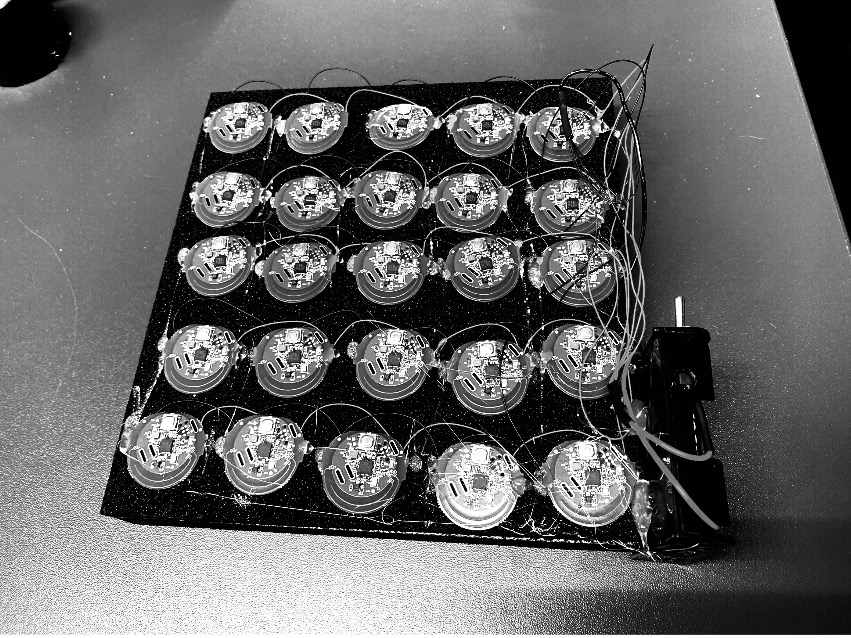
\includegraphics[width=7cm]{foculator}
\caption{Walkbase Foculator}
\label{fig:foculator}
\end{figure}

\begin{figure}[H]
\centering
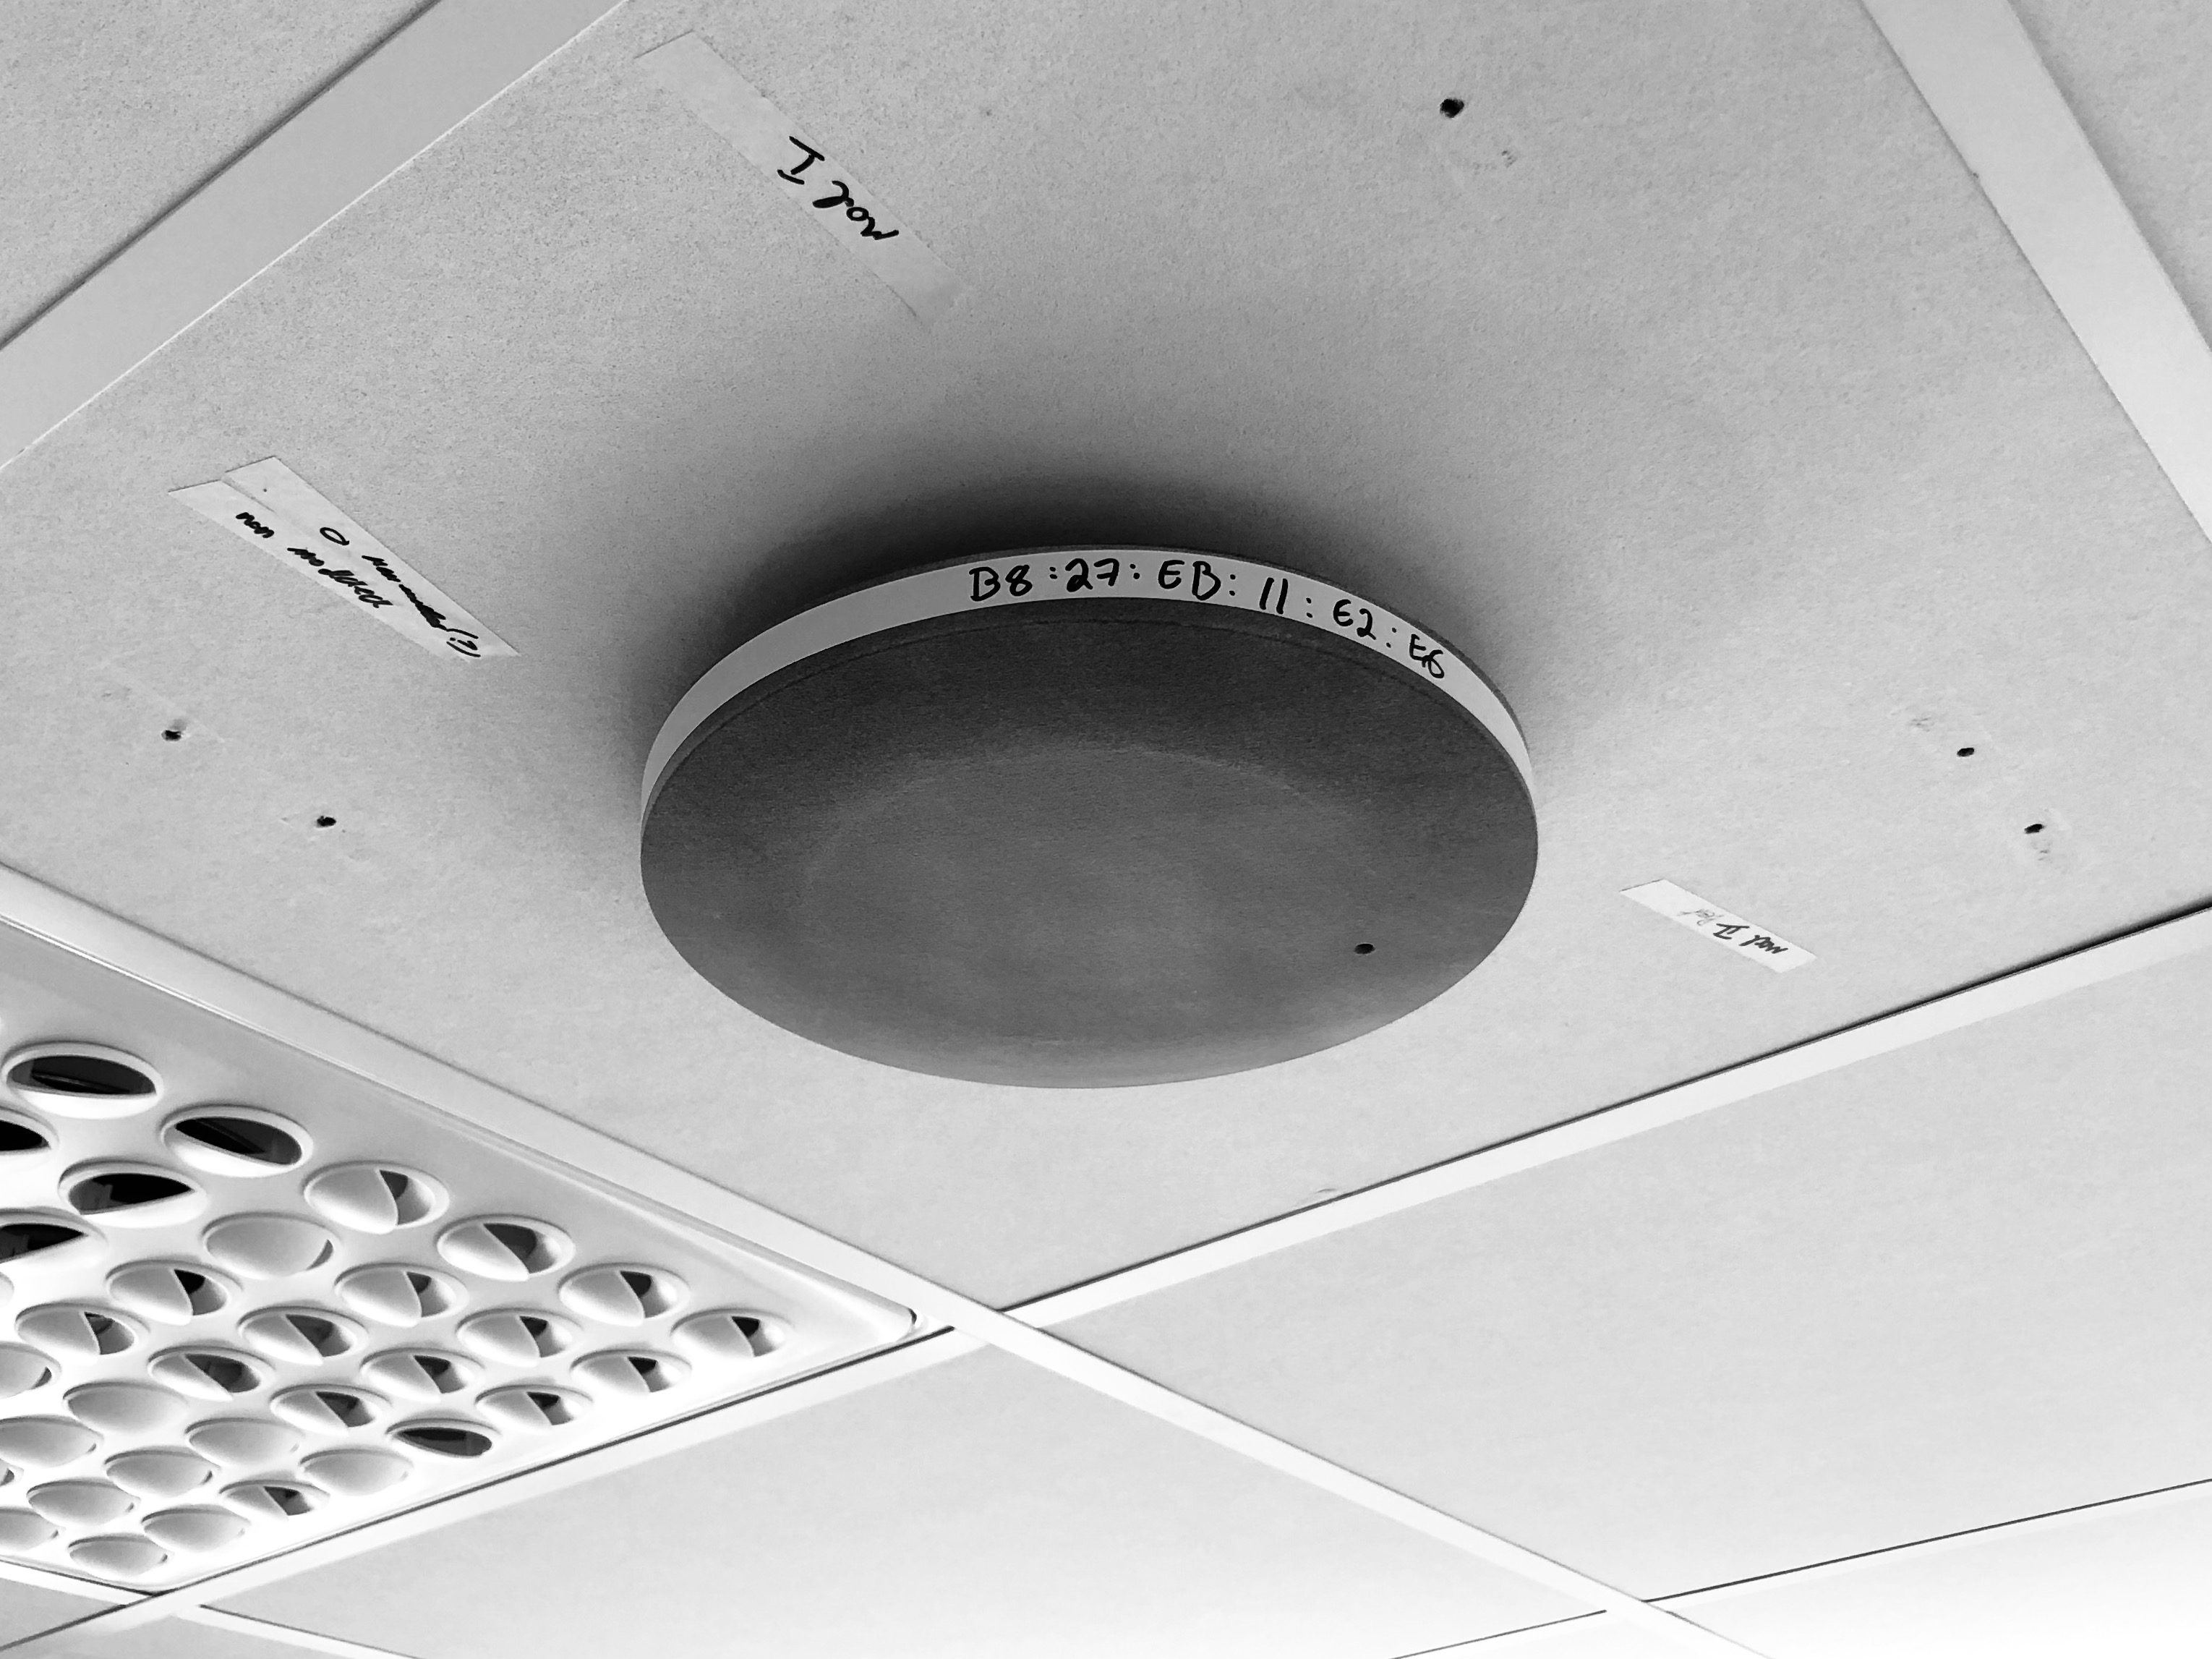
\includegraphics[width=7cm]{xr_2}
\caption{Walkbase XR-2}
\label{fig:xr2}
\end{figure}
\end{multicols}

Data on kuvattu tarkemmin alaluvussa 5.2. Koeympäristön pohjapiirustus on esitetty kuvassa \ref{fig:pohjapiirustus}. Piirustuksessa XR-2-paikantimet on kuvattu punaisilla numeroiduilla ympyröillä. Foculator-testilaitteen sijainti on kuvattu sinisellä ympyrällä. Toimistoympäristön pohjapiirustus on kuvattu harmaalla niin, että piirustuksesta erottuvat toimiston väliseinät.

\begin{figure}[H]
\centering
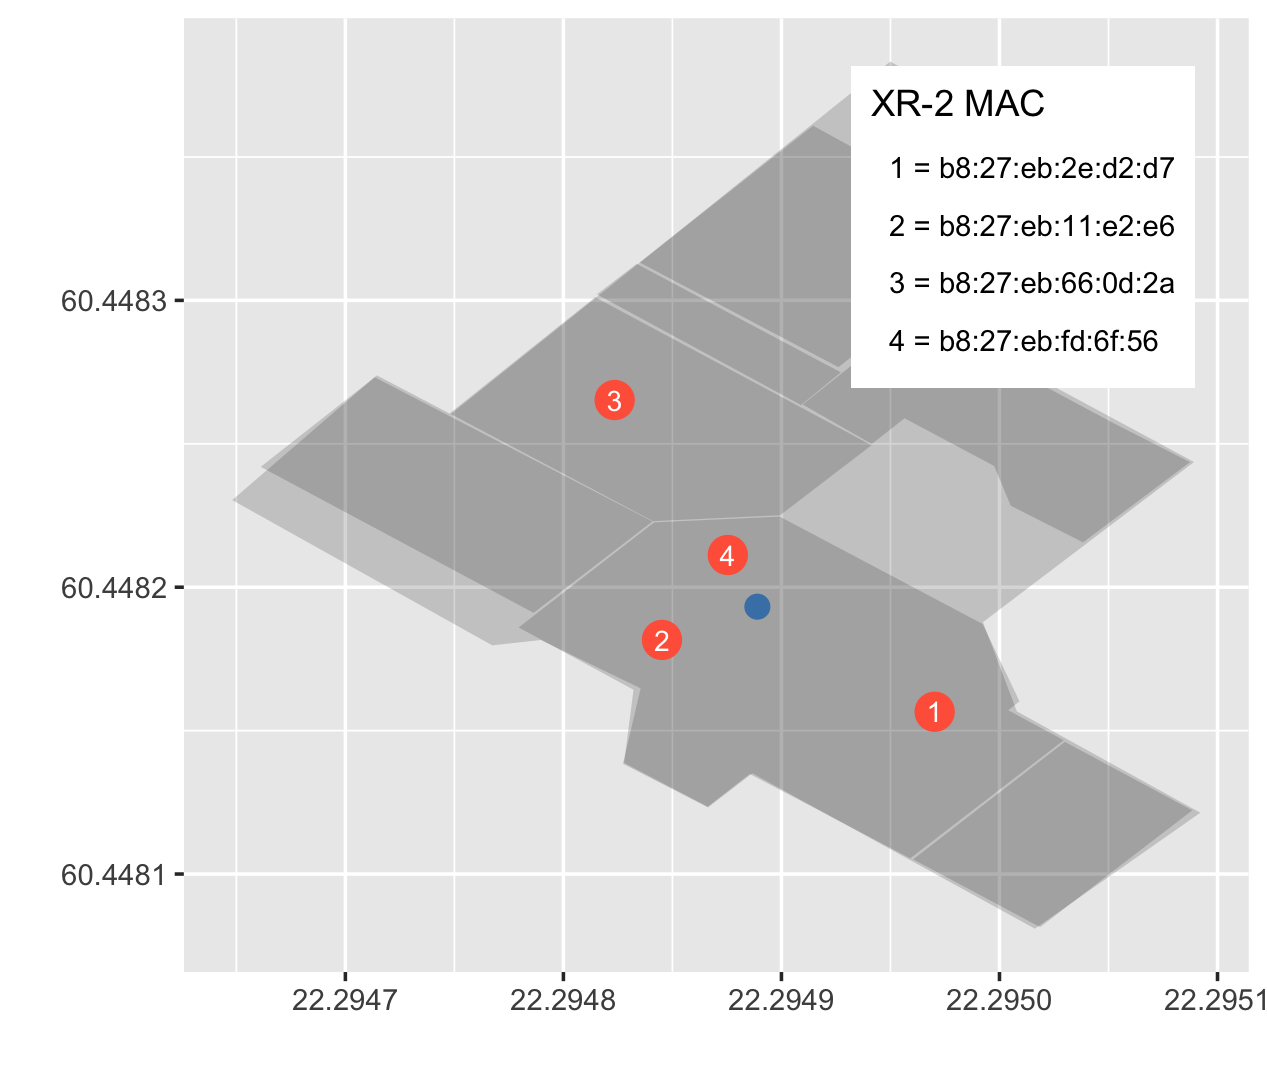
\includegraphics[width=12cm]{office_map}
\caption{Koeasetelman pohjapiirustus}
\label{fig:pohjapiirustus}
\end{figure}

\noindent Toimisto valittiin testiympäristöksi, koska siellä testaaminen on helpompaa ja halvempaa kuin aidossa kauppaympäristössä. Lisäksi toimistossa hyvin toimiva järjestelmä todennäköisesti toimii sellaisenaan vähemmän esteisessä kauppaympäristössä.

Dataa kerättiin sekä liikkuvalla että paikallaan olevalla testilaitteella. Paikallaan oleva testilaite asetettiin pöydälle 1.5 metrin korkeudelle. Liikkuvassa tapauksessa testilaite kiinnitettiin robottiin, joka oli ohjelmoitu seuraamaan haluttua liikerataa vastaavia lattiamerkintöjä ennalta määrätyllä vakionopeudella. Yksinkertaisuuden vuoksi tässä tutkielmassa tarkastellaan ainoastaan ongelmaa, jossa testilaite on paikoillaan. Esitetyt mallit soveltuvat kuitenkin myös liikkuvalle laitteelle. Data kerättiin yöaikaan, jolloin toimiston käyttöaste oli alhainen. Tällä minimoitiin radiosignaalien tielle osuvien ihmisten vaikutus signaaleihin. Maan pinnan kaarevuus on otettu huomioon koeasetelmassa pisteiden välisiä etäisyyksiä laskettaessa.

\section{Datan kuvaus}

Riippuen päällä olevien paikannustagien lukumäärästä sekä kulmaestimaattien luomiseen käytetystä laskentamenetelmästä tuottaa testilaite noin \(60\) havaintoa sekunnissa jokaista vastaanotinta kohden. Koetta varten käytettiin yhden minuutin aikana kertyneitä havaintoja. Havaintoja on datassa yhteensä \(N_{obs}=15018\) kappaletta. Havaintojen aikaleimat on tallennettu sekunnin tuhannesosan tarkkuudella. Jokainen havainto koostuu taulukossa \ref{tab:muuttujat} kuvatuista muuttujista.

\def\arraystretch{1.25} 
\begin{table}[H]
\centering
\begin{tabular}{|l|l|l|}
\hline
Muuttuja & Kuvaus & Esimerkkiarvo\\
\hline
ts & havainnon aikaleima & 21:38:20.998+00\\
locator\_mac & vastaanottimen MAC-osoite & b8:27:eb:66:0d:2a\\
azimuth\_angle & atsimuuttikulma $\theta$ (astetta) & 102.7\\
converted\_azimuth & napapohjoisesta laskettu kulma $\Phi$ (astetta) & 34\\
\makecell[tl]{snr\_ss} & \makecell[tl]{antennikohtaisten signaali-kohinasuhteiden\\neliösumma} & \makecell[tl]{6996.473}\\
rssi & signaalin vahvuus (dBm) & -81\\
distance & arvioitu etäisyys lähettimeen (m) & 13.5\\
\makecell[tl]{opposite\_angle} & \makecell[tl]{vastakkainen kulma\\ (lähetin-vastaanotin) $\Phi^\prime$ (radiaania)} & \makecell[tl]{3.735}\\
lat & vastaanottimen sijainti (leveyspiiri) & 60.448265\\
lon & vastaanottimen sijainti (pituuspiirit) & 22.294823\\
bearing & suuntimakulma $\eta$ (astetta) & 34\\
height & vastaanottimen korkeus (m) & 2.22 \\
\hline
\end{tabular}
\caption{Havaintomuuttujat}
\label{tab:muuttujat}
\end{table}

Etäisyys on estimoitu signaalin vahvuudesta käyttäen valmistajan omaa propagaatiomallia. Etäisyyttä tai signaalin vahvuutta ei käytetä paikantamiseen, joten tämän mallin käsittely jätetään tutkielman ulkopuolelle. Munoz (2009) luku 2 sisältää yleiskatsauksen propagaatiomalleista.

Atsimuuttikulma \(\phi\) lasketaan aina vastaanottimen tietyltä sivulta, joten se vastaa napapohjoista ainoastaan siinä tapauksessa, että vastaanottimen kyseinen sivu on asetettu kohtisuoraan napapohjoiseen nähden. Käytännön syistä tämä ei ole aina mahdollista eikä vaihe-erojen mittaamisen kannalta edes suotavaa. Tämän vuoksi jokaiselle vastaanottimelle on tietokantaan tallennettu oma suuntimakulma \(\eta\). Kokeessa käytetään napapohjoisesta laskettuja kulmia \(\Phi\), jotka lasketaan jokaiselle havainnolle havainnon vastaanottimen suuntimakulman avulla

\begin{align}
\Phi=(\theta + \eta+360^\degree) \mod360^\degree.
\end{align}

Suuntimakulma \(\Phi\) kertoo vastaanottimen ja lähettimen välisen kulman. Koska triangulaatiossa tarvitaan päinvastaista kulmaa, lasketaan lisäksi yhtälöllä (\ref{vastakkainen-kulma}) suuntimakulman perusteella lähettimen ja vastaanottimen välinen kulma \(\Phi^\prime\). Samalla asteissa oleva kulma muunnetaan radiaaneiksi triangulaatiota varten.

\begin{align}\label{vastakkainen-kulma}
\Phi^\prime=\frac{\pi}{180^\degree}(\Phi+180^\degree \mod360^\degree).
\end{align}

Lisäksi havainnot sisältävät antennikohtaisista SNR-arvoista lasketun neliösumman, jota käytetään erityisesti triangulaatiossa vahvimpien havaintojen valitsemiseen. Havaintomuuttujien ohella koetilanteessa tallennettiin Foculator-testilaitteen todellinen sijainti sekunnin tarkkuudella. Tallennettu sijainti perustuu koeympäristön lattiaan pohjapiirrustusten sekä laser-mittausten avulla tehtyihin merkintöihin. Näin saadut testimuuttujat on kuvattu taulukossa (\ref{tab:testimuuttujat}). Kun testilaite on paikoillaan, ovat nämä havainnot luonnollisesti samat jokaiselle ajanhetkelle.

\def\arraystretch{1.25} 
\begin{table}[H]
\centering
\begin{tabular}{|l|l|l|}
\hline
Muuttuja & Kuvaus & Esimerkkiarvo\\
\hline
foculator\_ts & aikaleima & 21:38:20+00\\
foculator\_lat & testilaitteen sijainti (leveyspiiri) & 60.44819 \\
foculator\_lon & testilaitteen sijainti (pituuspiiri) & 22.29493 \\
\hline
\end{tabular}
\caption{Testimuuttujat}
\label{tab:testimuuttujat}
\end{table}

\noindent Testimuuttujia käytetään paikannusalgoritmien paikannusvirheen laskemisessa.

\section{Ongelman kuvaus}

Tarkoituksena on estimoida testilaitteen/robotin sijainti sekunnin tarkkuudella. Merkitään estimoitavaa tilasarjaa \(x_{1:k}=\{x_1,\ldots,x_k\}\). Lisäksi merkitään \(x_0\) testilaitteen lähtösijaintia. Jokainen tilasarjan havainto koostuu suuntimakulmasta sekä pituus- että leveyskoordinaateista \((x_k^x, x_k^y)\). Määritellään tilalle testilaitteen/robotin kulkua kuvaava vektorisuunnistukseen (dead reckoning) perustuva malli (\ref{tilamalli-liikkuva})

\begin{align}\label{tilamalli-liikkuva}
x_{k+1}=f(x_k, \nu_k)=x_k+D_k \begin{bmatrix} \cos\psi_k \\ \sin\psi_k \end{bmatrix}+\nu_k,
\end{align}

\noindent missä \(D_k\) on testilaitteen/robotin ajanhetkenä \(k\) kulkema matka ja \(\psi_k\) testilaitteen/robotin atsimuutti/suuntimakulma kyseisenä ajanhetkenä. \(\nu_k\) on kohinaa, joka syntyy mittausvirheestä ja jolle voidaan olettaa \(\sim \mathcal{N}(\mu_x,\,\sigma_x^{2})\). Kun laite on paikallaan, yksinkertaistuu malli muotoon \(x_{k+1}=f(x_k)=\text{id}(x_k)=x_k\), missä \(\text{id}(\cdot)\) on identiteettifunktio.

Vastaavasti \(y_{1:k}=\{y_1,\ldots,y_k\}\) kuvaa paikantimien ja lähettimien välillä laskettuja kulmahavaintoja. Näin ollen jokainen havainto koostuu (maksimissaan) paikantimien määrää vastaavasta neljästä kulmasta. Havainnot lasketaan sekunnin tarkkuudella, mutta todellinen havaintotarkkuus on tiheämpi. Tästä syystä jokaisen sekunnin sensorihavainnot \(\{s_k^1,\ldots,s_k^4\}\) muodostetaan keskiarvona kaikista kyseisen sekunnin aikana tapahtuvista paikannin-lähetinparien kulmahavainnoista

\begin{align}
y_k=\begin{bmatrix} \frac{1}{n}\sum_{j=1}^ns^1_{k_j}\\   \vdots \\ \frac{1}{n}\sum_{j=1}^ns^4_{k_j} \end{bmatrix}.
\end{align}

\noindent Lisäksi tunnetaan sensoreihin \(\{s^1,\ldots,s^4\}\) liittyvät pituus- ja leveyskoordinaatit \((\lambda, \phi)\)

\begin{align}
u=\begin{bmatrix} \lambda^1 & \phi^1 \\   \vdots & \vdots \\ \lambda^4 & \phi^4 \end{bmatrix}.
\end{align}

Määritellään havainnoille malli

\begin{align}\label{havaintomalli}
y_k=h(x_k, u)+e_k=\text{atan2}(\begin{bmatrix}\phi^1-x_k^y\\ \vdots \\ \phi^4-x_k^y\end{bmatrix}, \begin{bmatrix}\lambda^1-x_k^x\\ \vdots \\ \lambda^4-x_k^x\end{bmatrix})+e_k,
\end{align}

\noindent missä

\begin{align}\label{atan2}
\displaystyle \operatorname{atan2}(y,x)={\begin{cases}\arctan({\frac {y}{x}})&{\text{jos }}>0,\\\arctan({\frac {y}{x}})+\pi &{\text{jos }}<0{\text{ ja }}y\geq 0,\\\arctan({\frac {y}{x}})-\pi & {\text{jos }}>0{\text{ ja }}<0,\\+{\frac {\pi }{2}}&{\text{jos }}x=0{\text{ ja }}>0,\\-{\frac {\pi }{2}}&{\text{jos }}x=0{\text{ ja }}<0,\\{\text{ei määritelty}}&{\text{jos }}x=0{\text{ ja }}y=0\end{cases}}
\end{align}

\noindent ja kohina noudattaa moniulotteista normaalijakaumaa \(e_k\sim\mathcal{N}(0,{\Sigma})\).

Kovarianssimatriisin estimaattina käytetään kunakin ajanhetkenä \(k\) antennikohtaisista havainnoista estimoituja otosvariansseja \(\text{diag}(\hat{\sigma}^1_k,\ldots,\hat{\sigma}^4_k)^2=\text{diag}(\frac{1}{n-1}\sum_{i=1}^n(s_i^1-\bar{s})^2,\ldots,\sum_{i=1}^n(s_i^4-\bar{s})^2)\). Määrittelemätön \(\text{atan2}\)-tapaus, jossa \(x=0\) ja \(y=0\) on käytetyllä mittaustarkkuudella käytännössä mahdoton. Jos tapaus halutaan välttää, voidaan nolla-arvot tarpeen vaatiessa korvata joillakin hyvin lähellä nollaa olevalla arvolla. Saadaan uskottavuusfunktioksi

\begin{align}
p(y_k|x_k)\propto\prod_{j=1}^4\exp\left\{-\frac{\norm{h(x^j_k,u)-y^j_k}^2}{2(\hat{\sigma}_i^j)^2}\right\},
\end{align}

\noindent missä \(j=\{1,2,3,4\}\) vastaa nyt kutakin XR-2-vastaanotinta.

Kumpikaan funktiosta \(h(\cdot)\) ja \(f(\cdot)\) ei ole lineaarinen, joten SIR-algoritmi on sopiva valinta ongelman ratkaisemiseksi. Koetuloksia arvioidaan ensisijaisesti paikannusvirheen avulla. Paikannusvirhe \(e_k\) lasketaan jokaisen ajanhetken \(k\) posteriorijakaumaestimaatista \(\hat{p}_k\) painotettuna keskiarvona

\begin{align}
\epsilon_k = \sum_{i=1}^Nw^k_i d(x^i_k, y_k),
\end{align}.

\noindent missä \(w_i^k\) on ajanketken \(k\) partikkelien normalisoitu paino ja \(d(x^i_k,y_k)\) partikkelien ja testilaitteen todellisen sijainnin välisen etäisyyden laskeva funktio.

\section{Algoritmin toteutuksesta}

Koeasetelmassa käytetty SMC-algoritmi on toteuttu R-kielellä. Algoritmin toteutus on pääosin vektorisoitu ja tehokas. For-silmukkaa on käytetty ainoastaan ajanhetkien läpikäyntiin. Koska tämän silmukan muuntaminen vektorisoituun muotoon ei ole mahdollista, voidaan toteutusta pitää näiltä osin hyvin optimoituna. Algoritmin rungon datan käsittely on toteutettu suorituskyvyltään hyvällä \texttt{data.table}-kirjastolla. Uskottavuusfunktiossa on käytetty hitaampia \texttt{dpylr}-kirjaston \texttt{tibble}-taulukkoja. Toteutustapa on valittu koodin ymmärrettävyyden parantamiseksi ja on edelleen riittävän nopea koeasetalman tarpeisiin. Koodin profilointi paljastaa, että suurin yksittäinen osa algoritmin ajasta kuluu \texttt{tibble}-taulukkojen käsittelyssä, joten suorituskykyä on tarpeen vaatiessa mahdollista myös parantaa.

Koska algoritmin uskottavuudet sekä painot ovat hyvin pieniä, on laskentatarkkuusongelmien välttämiseksi toteutuksessa käytetty logaritmoituja painoja ja uskottavuusfunktiota. Tämä ei vaikuta lainkaan itse algoritmin toimintaan, mutta estää numeeristen ongelmien syntymisen. Tilanteessa, jossa tietyn paikantimen ja kaikkien partikkelien välinen uskottavuus on nolla, päätyvät kaikki painot nolliksi eikä algoritmi enää toimi. Tällaisessa tilanteessa uskottavuusfunktion R-toteutus kutsuu itseään rekursiivisesti uudelleen niin, että kyseinen paikannin on tiputettu havainnoista.

Paikannusvirheen laskemisessa on etäisyysfunktiona \(d(\cdot)\) käytetty \texttt{raster}-kirjaston \texttt{pointDistance()}-funktiota. Koodissa on korostettu tiiviyden sijaan luettavuutta ja koodi on kommentoitu kattavasti. SMC-algoritmifunktion sekä uskottavuusfunktion R-koodit löytyvät osoitteesta \url{https://github.com/rintakumpu/luk}, mistä löytyy myös asetelmassa käytetty data csv-muodossa sekä kokeen muun koodin sisältävä R Markdown -notebook.

\section{Parametrien valinta}

Priorijakaumana \(p_{x_0}\) käytettiin kahta toisistaan riippumatonta otosta tasajakaumista, joista toinen vastasi leveys- ja toinen pituusasteita. Jakaumien alkupisteet valittiin niin, että ne vastasivat pienimpiä paikantimien leveys- ja pituusasteista. Vastaavasti päätepisteet valittiin niin, että ne vastasivat suurimpia paikantimien leveys- ja pituusasteita.

\begin{align}
&p_{x_{0_{\text{lon}}}}\sim\mathcal{U}(\min{\lambda},\max{\lambda}),\\
&p_{x_{0_{\text{lat}}}}\sim\mathcal{U}(\min{\phi},\max{\phi}).
\end{align}

\noindent Koska järjestelmän on tarkoitus toimia ainoastaan paikantimien muodostaman suorakaiteen sisäpuolella, ovat valitut jakaumien päätepisteet riittävät. Kummastakin jakaumasta otettiin \(\sqrt{N}\) otosta, jolloin \(N\) partikkelia \(x^i_0\) saatiin näiden otosten permutaatioina.

Paikannus suoritettiin yhteensä 17 kertaa. Ensimmäisessä vaiheessa tarkasteltiin partikkelien määrän \(N\) vaikutusta paikannuskeskivirheeseen ilman uudelleenotantaa sekä priori- että uskottavuusotannalla. Seuraavassa vaiheessa valittiin ehdotusjakauma edellisen vaiheen tulosten perusteella ja tarkasteltiin tilannetta sekä adaptiivisella että jokaisella iteraatiolla suoritettavalla uudelleenotannalla.

Kaikkien tulosten vertailukohtana käytettiin Pierlot \&al.~artikkelissa ``A New Three Object Triangulation Algorithm Based on the Power Center of Three Circles'' (2011) esittämää ToTal-triangulaatioalgoritmia. Triangulaatio-algoritmia ei käsitellä tässä tarkemmin, mutta se on esitetty algoritmissa \(\ref{total}\). Algoritmia varten valittiin kunakin ajanhetkenä \(k\) ne kolme paikanninta ja kulmahavaintoa, joiden SNR-arvo oli korkein.

Algoritmit ajettiin RStudion versiossa 1.4.1106 R-ohjelmointikielen versiolla 4.0.4. Tietokoneena käytettiin vuoden 2017 mallia olevaa MacBook Pro -kannettavaa, jossa oli 3.1 Ghz Quad-Core i7 -prosessori sekä 16 gigatavua 2133 Mhz LPDDR3 -muistia. Suoritusnopeuden mittaamiseen käytettiin \texttt{microbenchmark}-kirjastoa. Jokainen algoritmi toistettiin kymmenen kertaa ja suoritusnopeus laskettiin näiden toistojen aritmeettisena keskiarvona.

\section{Teknologian kuvaus}

Here is an equation.

\begin{equation} 
  f\left(k\right) = \binom{n}{k} p^k\left(1-p\right)^{n-k}
  \label{eq:binom}
\end{equation}

You may refer to using \texttt{\textbackslash{}@ref(eq:binom)}, like see Equation \eqref{eq:binom}.

\subsection{Kalibraatioalgoritmi}

\section{AoA-menetelmistä}

\subsection{MUSIC-algoritmi}

Footnotes are put inside the square brackets after a caret \texttt{\^{}{[}{]}}. Like this one \footnote{This is a footnote.}.

Citations. Reference items in your bibliography file(s) using \texttt{@key}.

For example, we are using the \textbf{bookdown} package \citep{R-bookdown} (check out the last code chunk in index.Rmd to see how this citation key was added) in this sample book, which was built on top of R Markdown and \textbf{knitr} \citep{xie2015} (this citation was added manually in an external file book.bib).
Note that the \texttt{.bib} files need to be listed in the index.Rmd with the YAML \texttt{bibliography} key.

The RStudio Visual Markdown Editor can also make it easier to insert citations: \url{https://rstudio.github.io/visual-markdown-editing/\#/citations}

\hypertarget{datan-kuvaus}{%
\section{Datan kuvaus}\label{datan-kuvaus}}

\hypertarget{ongelman-ja-mallien-kuvaus}{%
\section{Ongelman ja mallien kuvaus}\label{ongelman-ja-mallien-kuvaus}}

\hypertarget{datan-valinta}{%
\subsection{Datan valinta}\label{datan-valinta}}

Convex hull goes here.

\hypertarget{uskottavuusmallit}{%
\subsection{Uskottavuusmallit}\label{uskottavuusmallit}}

\hypertarget{dynaaminen-malli}{%
\subsection{Dynaaminen malli}\label{dynaaminen-malli}}

\hypertarget{algoritmien-toteutuksesta}{%
\section{Algoritmien toteutuksesta}\label{algoritmien-toteutuksesta}}

\hypertarget{karttasovitusalgoritmi}{%
\section{Karttasovitusalgoritmi}\label{karttasovitusalgoritmi}}

\hypertarget{reitinhakualgoritmi}{%
\section{Reitinhakualgoritmi}\label{reitinhakualgoritmi}}

\hypertarget{parametrien-valinnasta}{%
\section{Parametrien valinnasta}\label{parametrien-valinnasta}}

\hypertarget{tulokset}{%
\section{Tulokset}\label{tulokset}}

\hypertarget{lopuksi}{%
\chapter{Lopuksi}\label{lopuksi}}

Tässä tutkielmassa on esitetty pääpiirteittäin SMC-menetelmien teoria Bayesilaisessa tilastotieteellisessä viitekehyksessä. Lisäksi tutkielmassa on käyty läpi uudelleenotantaa efektiivisen otoskoon perusteella hyödyntävä SIR-suodinalgoritmi. Lopuksi tutkielmassa on tarkasteltu SIR-algoritmin parametrien valintaan, suorituskykyyn sekä konvergenssiin liittyviä tuloksia.

Tutkielmassa on lisäksi tarkasteltu miten eri valinnat vaikuttavat algoritmin suorituskykyyn yksinkertaisen mutta kattavan ja todelliseen ongelmaan sekä dataan perustuvan paikannusesimerkin avulla.

\begin{comment}
\begin{thebibliography}{99}
\bibitem{Cappe2007} Cappé, O., Godsill, S. J., Moulines, E., 2007. An Overview of Existing Methods and Recent Advances in Sequential Monte Carlo. \textit{Proceedings of the IEEE}, Vol 95, No 5, 899\textendash 924.
\bibitem{Crisan2014} Crisan, D. 2014. The stochastic filtering problem: A brief historical account. \textit{Journal of Applied Probability}, Vol 51(A), 13\textendash 22.
\bibitem{Crisan2000} Crisan, D., Doucet, A. 2000. \textit{Convergence of Sequential Monte Carlo Methods}. 
\bibitem{Crisan2002} Crisan, D., Doucet, A. 2002. A survey of convergence results on particle filtering methods for practitioners. \textit{IEEE Transactions on Signal Processing}, Vol 50, No 3, 736\textendash 746.
\bibitem{Davidson2010} Davidson, P., Collin J., Takala J. 2010, Application of particle filters for indoor positioning using floor plans. \textit{2010 Ubiquitous Positioning Indoor Navigation and Location Based Service}, 1\textendash 4.
\bibitem{DelMoral1996} Del Moral, P. 1997. Nonlinear filtering: Interacting particle resolution. \textit{Markov Processes and Related Fields}, Vol 2, No 4, 555\textendash 580.
\bibitem{Gordon1993} Gordon, N.J., Salmond, D.H., Smith A.F.M. 1993. Novel approach to
nonlinear/non-Gaussian Bayesian state estimation. \textit{IEE Proc. F, Radar Signal Process}, Vol 140, No 2, 107\textendash 113.
\bibitem{Grewal2010} Grewal, M.S., Andrews, A.P. 2010. Applications of Kalman Filtering in Aerospace 1960 to the Present [Historical Perspectives]. \textit{IEEE Control Systems Magazine}, Vol 30, No 3, 69\textendash 78.
\bibitem{Gustafsson2010} Gustafsson, F. 2010. Particle filter theory and practice with positioning applications. \textit{IEEE Aerospace and Electronic Systems Magazine}, Vol 25, No 7, 53\textendash 82.
\bibitem{LiuChen1998} Liu, J., Chen, R. 1998. Sequential Monte Carlo Methods for Dynamic Systems. \textit{Journal of the American Statistical Association}, Vol 93, No 443, 1032\textendash 1044.
\bibitem{Munoz2009} Munoz, D., Enriquez-Caldera, R., Vargas, C., Bouchereau Lara, F. 2009. \textit{Position Location Techniques and Applications}. Elsevier.
\bibitem{Pierlot2011} Pierlot, V., Urbin-Choffray M., Van Droogenbroeck, M. 2011. A New Three Object Triangulation Algorithm Based on the Power Center of Three Circles. \textit{Research and Education in Robotics - EUROBOT 2011}, 248\textendash 262. Springer.
\bibitem{Sarkka2013} Särkkä, S. 2013. \textit{Bayesian Filtering and Smoothing}. Cambridge University Press.
\end{thebibliography}
\end{comment}

\hypertarget{liite-other-stuff--followed-by-a-chapter}{%
\chapter{\texorpdfstring{(Liite) Other stuff \{-\}\texttt{(followed\ by}\# A chapter`)}{(Liite) Other stuff \{-\}(followed by\# A chapter`)}}\label{liite-other-stuff--followed-by-a-chapter}}

  \bibliography{packages.bib}

\end{document}
